\documentclass[10pt]{beamer}

%%%
% PREAMBLE FOR THIS DOC 
%%%
%https://tex.stackexchange.com/questions/68821/is-it-possible-to-create-a-latex-preamble-header
\usepackage{/Users/miw267/Repos/latex_preamble/beamer_preamble}

\usetikzlibrary{matrix}

\usetikzlibrary{shapes.geometric}

\usepackage{pgfplots} % For drawing histograms
\usetikzlibrary{pgfplots.groupplots} % For grouping multiple plots


%%%
% AGENDA TOPICS
%%%
\agendatopic[overview]{Overview}
\agendatopic[expectation]{Expectation}
\agendatopic[variance]{Variance}





%%%
% DOCUMENT
%%%

\begin{document}

%\maketitle

%% Title page frame
%\begin{frame}
%    \titlepage 
%\end{frame}



\title{11/13/2026: Expectation and Variance}
\author{CSCI 246: Discrete Structures}
\date{Textbook reference: Sec 34, Scheinerman}

\begin{frame}
    \titlepage 
\end{frame}


\begin{frame}


\begin{mygreenbox}[title=Graded Quiz Pickup]
Quizzes are in the front of the room, grouped into four bins (A-G, H-L, M-R, S-Z) by last name. The quizzes are upside down with your last name on the back. Come find yours before, during, or after class.  Only turn the quiz over if it's yours.
\end{mygreenbox} 
\vfill
\begin{myyellowbox}[title=Today's Agenda]
\begin{itemize}
	\item Quiz
	\item Mini-lecture 
	\item Group exercises
\end{itemize}
\end{myyellowbox}
\vfill 

\end{frame}



\begin{frame}{Quiz \#10}
\small 

\begin{enumerate}
	\item Let $(S,P)$ be the probability space for a single roll of a fair six-sided die. What is the sample space $S$? What is $P(s)$ for each outcome $s \in S$?
	\item  What is the probability of getting a \textbf{three of a kind} in a 5-card poker hand?      (Note: A \textit{three of a kind} refers to a poker hand where three cards have the same rank and the two other cards have different ranks.  For example, a hand with three 10s, a 7, and a jack is a three-of-a-kind.) 
	\item \textit{(Spinner Winner.)}  Below are two spinners. When you spin A, you have a 50\% chance of winning, and when you spin B, you have a 25\% chance of winning.  If you land on Win after a spin, you will win \$1 million.  Which of the following options is your best course of action? (a) Spin A once, (b) Spin B twice, so you get two shots, or (c) It makes no difference. Justify your answer using a probabilistic argument.
\end{enumerate}

\centering
\def\r{1.3}% radius of each spinner (cm): change this to resize
\begin{tikzpicture}[scale=0.75, every node/.style={font=\small}]
  % Spinner A
  \begin{scope}
    \fill[gray!40] (0,0) -- (90:\r) arc (90:-90:\r) -- cycle;
    \draw[thick] (0,0) circle (\r);
    \node at (180:0.6*\r) {Lose};
    \node at (0:0.6*\r) {Win};
    \draw[very thick, -latex] (270:0.55*\r) -- (90:0.85*\r);
    \fill (0,0) circle (0.07);
    \node[font=\large\bfseries] at (0,\r+0.4) {A};
  \end{scope}
  % Spinner B
  \begin{scope}[xshift={3*\r cm}]
    \fill[gray!40] (0,0) -- (0:\r) arc (0:90:\r) -- cycle;
    \draw[thick] (0,0) circle (\r);
    \node at (45:0.6*\r) {Win};
    \node at (225:0.5*\r) {Lose};
    \draw[very thick, -latex] (270:0.55*\r) -- (90:0.85*\r);
    \fill (0,0) circle (0.07);
    \node[font=\large\bfseries] at (0,\r+0.4) {B};
  \end{scope}
\end{tikzpicture}

\end{frame}


%%%%%%%%%%%%%%%
%%%%%%%%%%%%%%%
%%%%%%%%%%%%%%%
\agendaframe{overview}

%
%\begin{frame}{Expectations and variances in real life (1/2)}
%	
%\small 
%\textbf{Expectation} tells you the average value of a random variable.
%\vfill 
%\pause 
%\begin{myyellowbox}[title= Example of how expectations are useful]
%Two companies offer LSAT preparation for law school. You may want to choose the company that offers a larger expected increase in LSAT scores.
%\end{myyellowbox}
%
%
%\vfill 
%\pause 
%
%\textbf{Variance} tells you how much spread (or uncertainty) there is about a random variable.
%\vfill 
%\pause 
%
%
%\begin{mybluebox}[title= Example of how variances are useful]
% Two companies offer LSAT preparation for law school.  Both offer the same expected increase in LSAT score.   However, they differ in the variability of increases in LSAT scores.  (Company A has a larger spread in score boosts than company B.) 
% \begin{itemize}
% 	\item  If you want to minimize risk, you may want to choose company A.
% 	\item If you want to maximize potential gain, you may want to choose company B.
% \end{itemize}
%
%\end{mybluebox}
%
%\end{frame}

%\begin{frame}{Expectations and variances in real life (1/2)}
%
%\small 
%\textbf{Expectation} tells you the average value of a random variable.
%\vfill 
%\begin{myyellowbox}[title= Example of how expectations are useful]
%You can drive to campus by two routes.  You may want to choose the route with the shorter expected travel time.
%\end{myyellowbox}
%
%
%\vfill 
%\pause 
%
%\textbf{Variance} tells you how much spread (or uncertainty) there is about a random variable.
%\vfill 
%\pause 
%
%
%\begin{mybluebox}[title= Example of how variances are useful]
% Two routes both take 25 minutes on average.  But the highway usually takes 20 minutes and sometimes takes 45 (when there's an accident), while the back roads always take 24--26 minutes.  So the highway has a larger variance.
% \vspace{-.2cm}
% \begin{itemize}
% 	\item If you can't be late (e.g., for an exam), you may want to take the back roads.
% 	\item If you're willing to gamble for a quicker trip, you may want to take the highway.
% \end{itemize}
%
%\end{mybluebox}
%
%
%	
%\end{frame}




\begin{frame}{Expectations and variances in real life (1/2)}
\footnotesize

\begin{itemize}
\item \textbf{Expectation} tells you the average value of a random variable.
\item \textbf{Variance} tells you how much spread (or uncertainty) there is about a random variable.
\end{itemize}

\begin{myyellowbox}[title= \text{Example: The National Football League}]
Tight end Tony Gonzalez and wide receiver Torrey Smith both averaged about 8 yards per target. But Smith's boom-or-bust gains had about 3.5 times the variance.
\vfill \vfill 
\centering
\begin{minipage}{0.85\linewidth}
% photos centered over the player names (at 29.0% and 76.4% of the plot's width)
\begin{tikzpicture}[x=\linewidth]
  \useasboundingbox (0,-0.425cm) rectangle (1,0.425cm);
  \node[inner sep=0] at (0.290,0) {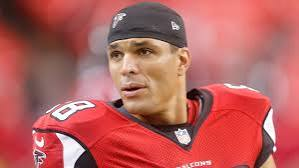
\includegraphics[height=0.85cm]{images/tony_gonzalez.jpeg}};
  \node[inner sep=0] at (0.764,0) {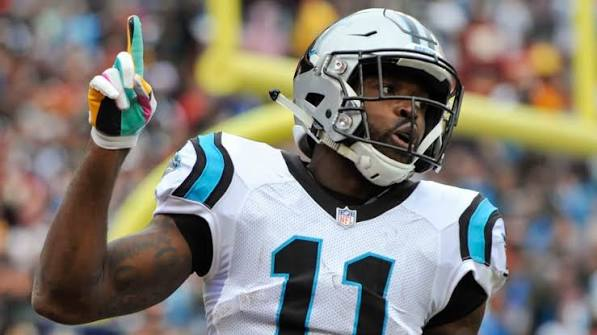
\includegraphics[height=0.85cm]{images/torrey.jpeg}};
\end{tikzpicture}

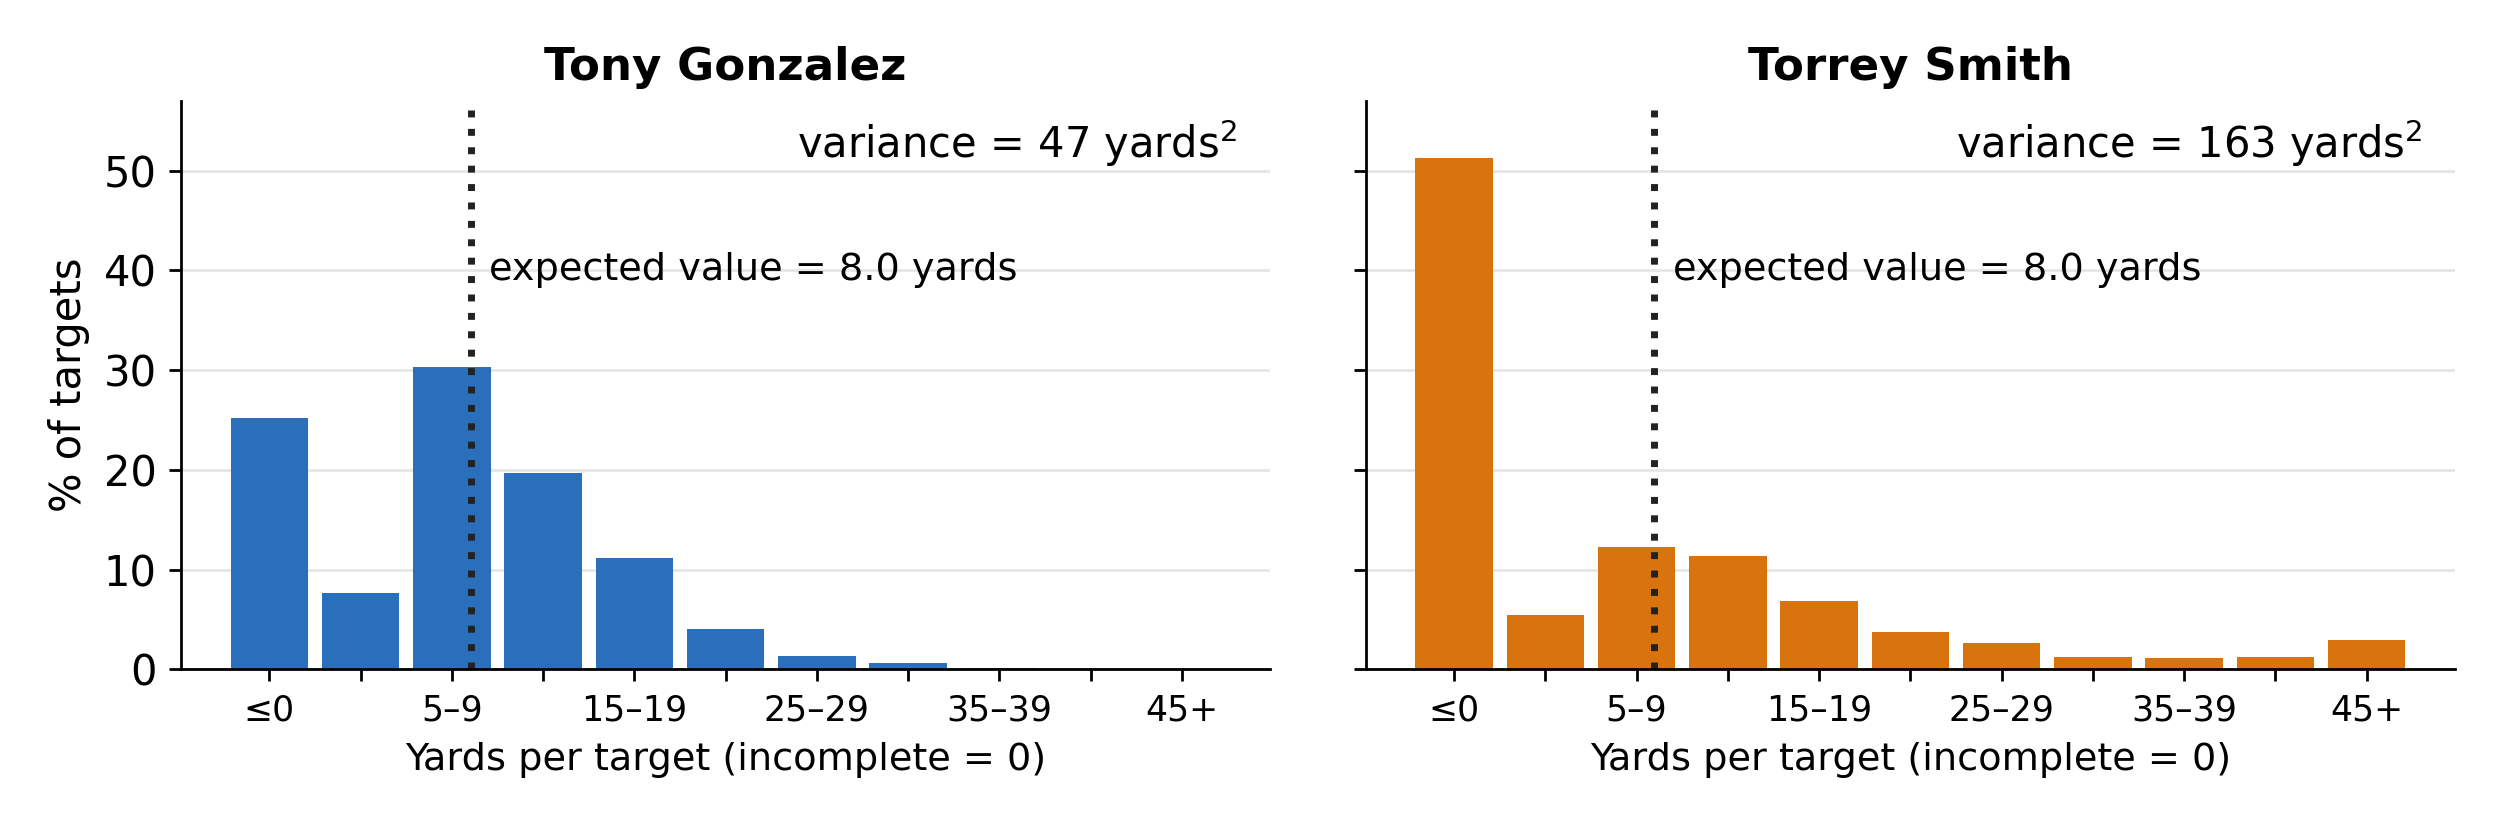
\includegraphics[width=\linewidth]{images/yards_per_target_gonzalez_smith_wide.png}
\end{minipage}
\vfill
\end{myyellowbox}
\pause 
Today, we'll practice computing these quantities from data.
\end{frame}



\begin{frame}{Expectations and variances in real life (2/2)}

\footnotesize



\begin{itemize}
\item \textbf{Expectation} tells you the average value of a random variable.
\item \textbf{Variance} tells you how much spread (or uncertainty) there is about a random variable.
\end{itemize}





\begin{myyellowbox}[title= \text{Example: Parking at MSU}]

\begin{minipage}{0.48\linewidth}

\begin{center}
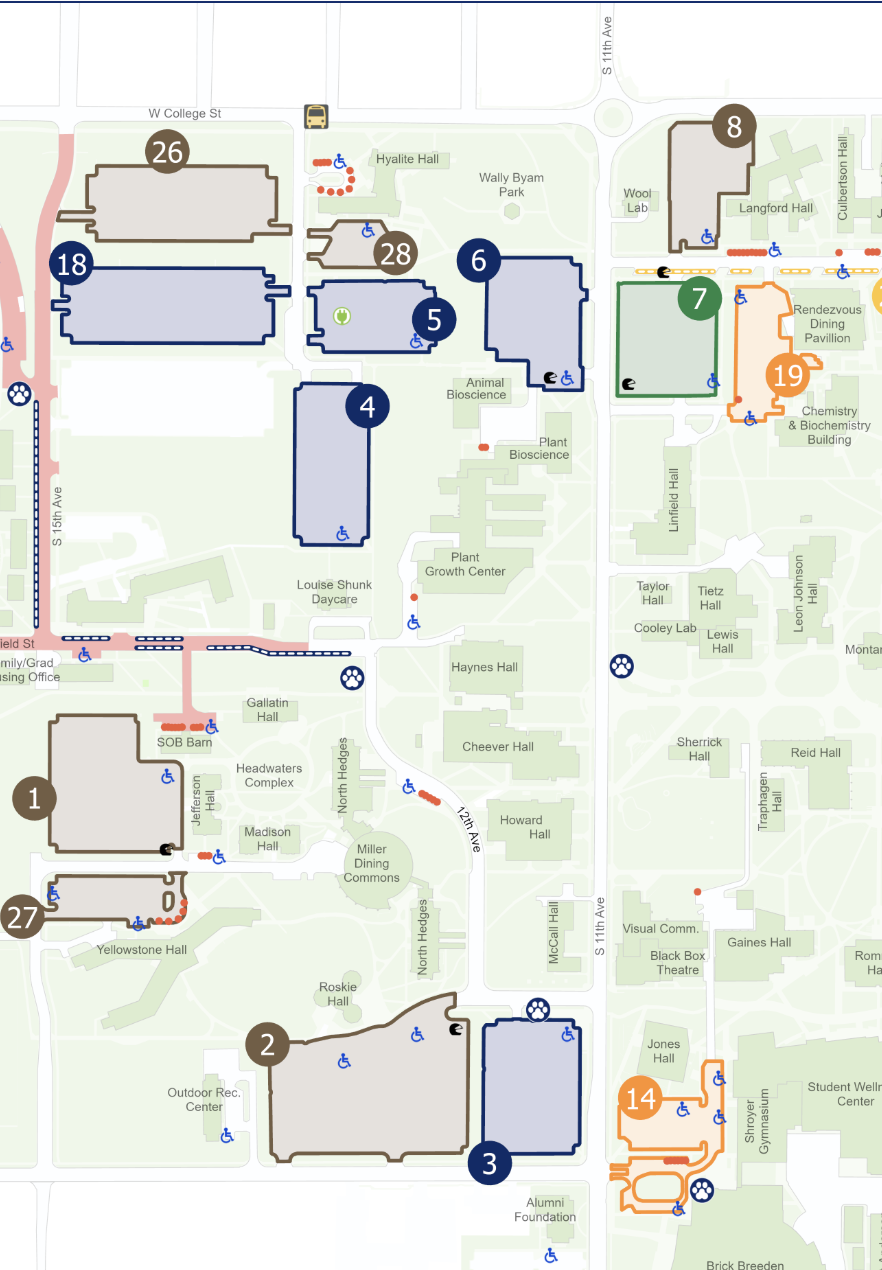
\includegraphics[width=.85\linewidth]{images/parking_lot_map}
\end{center}
\end{minipage} %
\begin{minipage}{0.48\linewidth}
\scriptsize 
Should I park in lot 18 or lot 3?   Lot 3 is closer to my destinations, but usually there's no parking spot open.  So I'll probably have to circle around for a long time.   
\begin{itemize}
\item My trip time has smaller expectation and smaller variance if I park at lot 18. So that's where I usually park. 
\item However, sometimes if I'm running late, I'll choose lot 3 \textbf{because} it has higher variance... Maybe I'll get lucky and make it on time.
\end{itemize}

	
\end{minipage} %



\end{myyellowbox}


	
\end{frame}




%%%%%%%%%%%%%%%
%%%%%%%%%%%%%%%
%%%%%%%%%%%%%%%
\agendaframe{expectation}


\begin{frame}

Suppose we roll a pair of dice.  What is the \textit{expected value} of the sum?
\vfill 
\begin{figure}

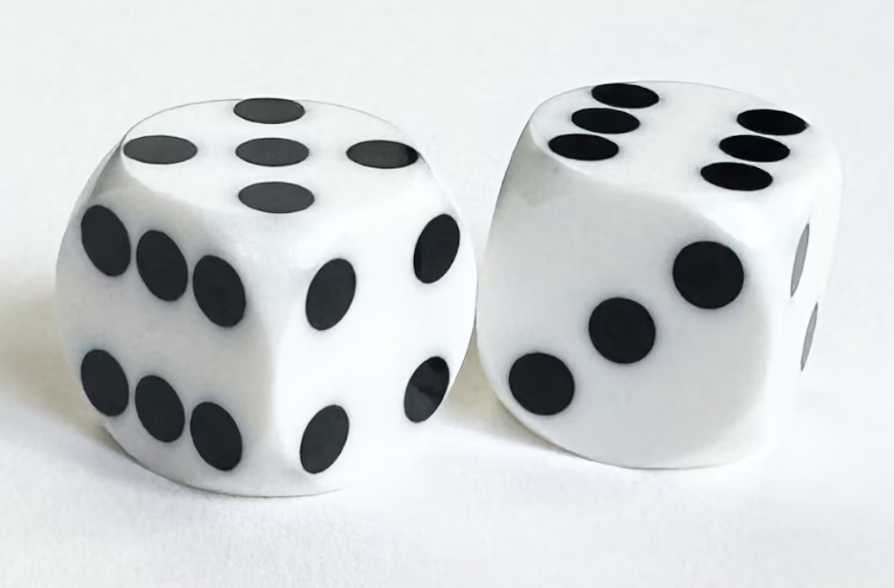
\includegraphics[width=.8\textwidth]{images/pair_of_dice.png}
\end{figure}
\vfill 
Formally, let $X$ be the sum of the number on the two dice.  We must compute $E[X]$.
	
\end{frame}

\begin{frame}{Computing An Expectation}
\footnotesize 
\begin{table}
\caption{\textit{Possible outcomes when rolling a pair of dice.} Each table entry gives the sum of the values on the two dice.}	
\pause 
\resizebox{0.6\textwidth}{!}{%
\begin{tabular}{|c|c|c|c|c|c|c|c|}
\hline
\textbf{Dice Values} & \textbf{1} & \textbf{2} & \textbf{3} & \textbf{4} & \textbf{5} & \textbf{6} \\
\hline
\textbf{1} & \cellcolor{red!20} 2  & \cellcolor{red!40} 3  & \cellcolor{red!60} 4  & \cellcolor{red!80} 5  & \cellcolor{red!90} 6  & \cellcolor{red!100} 7 \\
\hline
\textbf{2} & \cellcolor{red!40} 3  & \cellcolor{red!60} 4  & \cellcolor{red!80} 5  & \cellcolor{red!90} 6  & \cellcolor{red!100} 7  & \cellcolor{orange!80} 8 \\
\hline
\textbf{3} & \cellcolor{red!60} 4  & \cellcolor{red!80} 5  & \cellcolor{red!90} 6  & \cellcolor{red!100} 7  & \cellcolor{orange!80} 8  & \cellcolor{orange!60} 9 \\
\hline
\textbf{4} & \cellcolor{red!80} 5  & \cellcolor{red!90} 6  & \cellcolor{red!100} 7  & \cellcolor{orange!80} 8  & \cellcolor{orange!60} 9  & \cellcolor{orange!40} 10 \\
\hline
\textbf{5} & \cellcolor{red!90} 6  & \cellcolor{red!100} 7  & \cellcolor{orange!80} 8  & \cellcolor{orange!60} 9  & \cellcolor{orange!40} 10 & \cellcolor{orange!20} 11 \\
\hline
\textbf{6} & \cellcolor{red!100} 7 & \cellcolor{orange!80} 8 & \cellcolor{orange!60} 9 & \cellcolor{orange!40} 10 & \cellcolor{orange!20} 11 & \cellcolor{yellow!20} 12 \\
\hline
\end{tabular}
}
\end{table}

\vfill 
\pause 
\colorbox{blue!30}{\textbf{Method 1.}} \; Sum over outcomes in the sample space.
\[ E[X] = \sum_{s \in S} X(s) P(s) \]
\vfill 
\pause 
\colorbox{blue!30}{\textbf{Application.}}
\scriptsize 
\begin{align*}
 E[X] 
&=\colorbox{red!20}{1+1} \!\cdot\! \frac{1}{36} + \colorbox{red!40}{1+2}\!\cdot\!\frac{1}{36}  + \colorbox{red!40}{2+1} \!\cdot\! \frac{1}{36} +\colorbox{red!60}{3+1} \!\cdot\! \frac{1}{36}  + \colorbox{red!60}{2+2} \!\cdot\!\frac{1}{36}  + 
 \colorbox{red!60}{1+3} \!\cdot\!\frac{1}{36} + \hdots + 
  \colorbox{yellow!20}{6+6} \!\cdot\! \frac{1}{36}  \\
 &= \colorbox{red!20}{2} \cdot \frac{1}{36} + \colorbox{red!40}{3} \cdot \frac{1}{36}  + \colorbox{red!40}{3} \cdot \frac{1}{36} +\colorbox{red!60}{4} \cdot \frac{1}{36}  + \colorbox{red!60}{4} \cdot \frac{1}{36}  + 
 \colorbox{red!60}{4} \cdot \frac{1}{36} + \hdots + 
  \colorbox{yellow!20}{12} \cdot \frac{1}{36} 
\end{align*}
\footnotesize 
\vfill 
\pause 
\colorbox{blue!30}{\textbf{Remark.}} \; We must sum over \textbf{many} (36) terms.
\end{frame}


\begin{frame}{Computing An Expectation}
\footnotesize  
\begin{table}
\caption{\textit{Possible outcomes when rolling a pair of dice.} Each table entry gives the sum of the values on the two dice.}	
\begin{tabular}{|c|c|c|c|c|c|c|c|}
\hline
\textbf{Dice Values} & \textbf{1} & \textbf{2} & \textbf{3} & \textbf{4} & \textbf{5} & \textbf{6} \\
\hline
\textbf{1} & \cellcolor{red!20} 2  & \cellcolor{red!40} 3  & \cellcolor{red!60} 4  & \cellcolor{red!80} 5  & \cellcolor{red!90} 6  & \cellcolor{red!100} 7 \\
\hline
\textbf{2} & \cellcolor{red!40} 3  & \cellcolor{red!60} 4  & \cellcolor{red!80} 5  & \cellcolor{red!90} 6  & \cellcolor{red!100} 7  & \cellcolor{orange!80} 8 \\
\hline
\textbf{3} & \cellcolor{red!60} 4  & \cellcolor{red!80} 5  & \cellcolor{red!90} 6  & \cellcolor{red!100} 7  & \cellcolor{orange!80} 8  & \cellcolor{orange!60} 9 \\
\hline
\textbf{4} & \cellcolor{red!80} 5  & \cellcolor{red!90} 6  & \cellcolor{red!100} 7  & \cellcolor{orange!80} 8  & \cellcolor{orange!60} 9  & \cellcolor{orange!40} 10 \\
\hline
\textbf{5} & \cellcolor{red!90} 6  & \cellcolor{red!100} 7  & \cellcolor{orange!80} 8  & \cellcolor{orange!60} 9  & \cellcolor{orange!40} 10 & \cellcolor{orange!20} 11 \\
\hline
\textbf{6} & \cellcolor{red!100} 7 & \cellcolor{orange!80} 8 & \cellcolor{orange!60} 9 & \cellcolor{orange!40} 10 & \cellcolor{orange!20} 11 & \cellcolor{yellow!20} 12 \\
\hline
\end{tabular}
\end{table}

\vfill 

\colorbox{blue!30}{\textbf{Method 2.}} \;  Sum over possible values of the random variable.
\[ E[X] = \sum_{a \in \R} a \; P(X=a) \]
\vfill 
\pause 
\colorbox{blue!30}{\textbf{Application.}}
\begin{align*}
 E[X] &= \colorbox{red!20}{2} \cdot \frac{1}{36} + \colorbox{red!40}{3} \cdot \frac{2}{36}  +\colorbox{red!60}{4} \cdot \frac{3}{36}  +\hdots + 
  \colorbox{yellow!20}{12} \cdot \frac{1}{36} 
\end{align*}
\vfill 
\pause 
\colorbox{blue!30}{\textbf{Remark.}} \; We must sum over \textbf{fewer} (12) terms.
\end{frame}


\begin{frame}{Computing An Expectation}
\footnotesize  
\begin{table}
\caption{\textit{Possible outcomes when rolling a pair of dice.} Each table entry gives the sum of the values on the two dice.}	
\begin{tabular}{|c|c|c|c|c|c|c|c|}
\hline
\textbf{Dice Values} & \textbf{1} & \textbf{2} & \textbf{3} & \textbf{4} & \textbf{5} & \textbf{6} \\
\hline
\textbf{1} & \cellcolor{red!20} 2  & \cellcolor{red!40} 3  & \cellcolor{red!60} 4  & \cellcolor{red!80} 5  & \cellcolor{red!90} 6  & \cellcolor{red!100} 7 \\
\hline
\textbf{2} & \cellcolor{red!40} 3  & \cellcolor{red!60} 4  & \cellcolor{red!80} 5  & \cellcolor{red!90} 6  & \cellcolor{red!100} 7  & \cellcolor{orange!80} 8 \\
\hline
\textbf{3} & \cellcolor{red!60} 4  & \cellcolor{red!80} 5  & \cellcolor{red!90} 6  & \cellcolor{red!100} 7  & \cellcolor{orange!80} 8  & \cellcolor{orange!60} 9 \\
\hline
\textbf{4} & \cellcolor{red!80} 5  & \cellcolor{red!90} 6  & \cellcolor{red!100} 7  & \cellcolor{orange!80} 8  & \cellcolor{orange!60} 9  & \cellcolor{orange!40} 10 \\
\hline
\textbf{5} & \cellcolor{red!90} 6  & \cellcolor{red!100} 7  & \cellcolor{orange!80} 8  & \cellcolor{orange!60} 9  & \cellcolor{orange!40} 10 & \cellcolor{orange!20} 11 \\
\hline
\textbf{6} & \cellcolor{red!100} 7 & \cellcolor{orange!80} 8 & \cellcolor{orange!60} 9 & \cellcolor{orange!40} 10 & \cellcolor{orange!20} 11 & \cellcolor{yellow!20} 12 \\
\hline
\end{tabular}
\end{table}

\vfill 
\colorbox{blue!30}{\textbf{Method 3.}} \; Use linearity of expectation.
\[ E[X] = E[D_1] + E[D_2] \]
where $D_n$ is the value on the $n$-th die.
\vfill 
\pause 
\colorbox{blue!30}{\textbf{Application.}} We have 
\begin{align*}
 E[X] &= E[D_1] + E[D_2] = 3.5 + 3.5 = 7.
\end{align*}
%
since, by the previous methods, each $E[D_n] = \frac{1}{6} \cdot  (1+2+3+4+5+6) = 3.5$.

\vfill 
\pause 
\colorbox{blue!30}{\textbf{Remark.}} \; Here we can sum over \textbf{even fewer} (2 or 7) terms.   (Note: we can only use Method 3 in cases where we can express $X$ as a sum of other RVs).
\end{frame}


%\begin{frame}{Summary on computing an expectation}
%Some ways of computing the expectation are more efficient than others.
%\vfill 
%%Foreshadowing our upcoming section on computational complexity, we can make a more general statement: 
%%\vfill 
%
%\begin{myredbox}[title=\text{Remark: Scalability of different methods for computing an expectation}]
%Let $X$ be the sum of $n$ random variables each from the same sample space $S$.  Then the number of operations needed to compute $E[X]$ is
%\vfill 
%\begin{itemize}
%\item Method 1: $\Theta(|S|^n)$	, i.e. \textbf{exponential} in $n$.
%\item Method 2: $\Theta(n \, |S|)$, i.e. \textbf{linear} in $n$.
%\item Method 3: $\Theta(|S|)$,  i.e. \textbf{independent} of $n$.
%\end{itemize}
%\end{myredbox}
%
%%We will investigate computational complexity (and define $\mathcal{O}$) in a couple of class meetings.
%
%\end{frame}


\begin{frame}{Expectation as center of probability mass}
\footnotesize 
Consider a probability space $(S,P)$ where $S=\set{1,2,\hdots,10}$ and $P(s) =\frac{1}{10}$ for all outcomes $s \in S$.  Define a random variable $X$ as below:
\vfill 
\begin{figure}
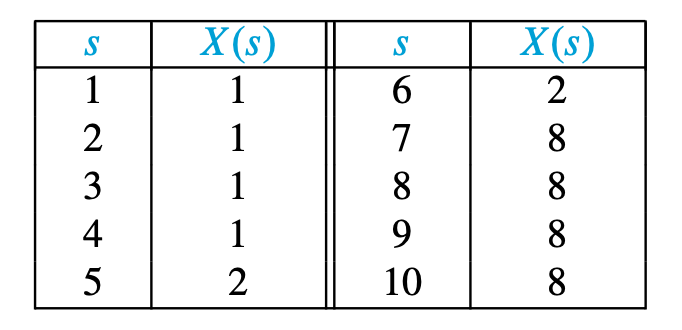
\includegraphics[width=.5\textwidth]{images/center_of_mass__table}
\end{figure}
\vfill 
Now we make a seesaw, placing a weight $P(X=a)$ for each outcome $a$ that the random variable can take on:
\begin{figure}
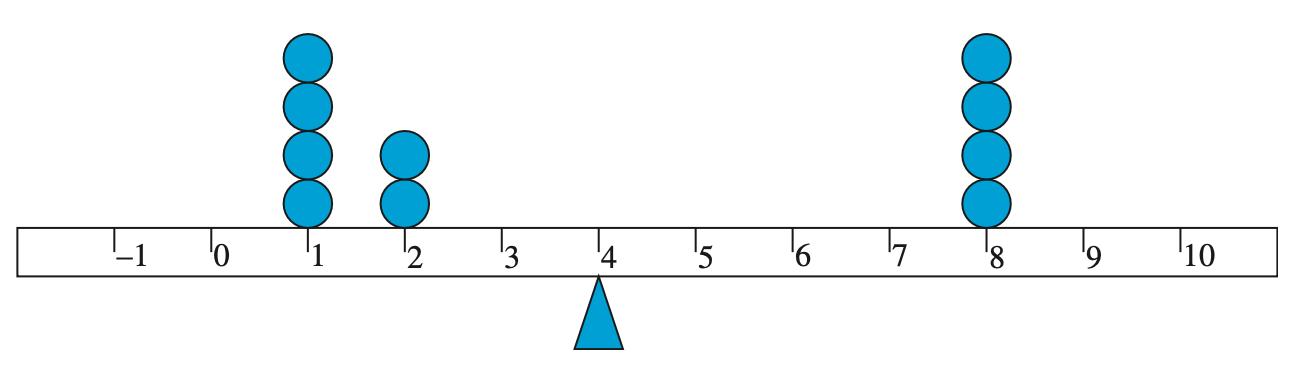
\includegraphics[width=.7\textwidth]{images/center_of_mass}
\end{figure}
%
What is the expected value? \pause The \textbf{balancing point} (\tikz[baseline=-0.5ex]{
    \fill[blue!80] (0,-0.2) -- (0.4,-0.2) -- (0.2,0.35) -- cycle;
}) of the seesaw!

\end{frame}

\begin{frame}{Expectation as center of probability mass}

\begin{figure}
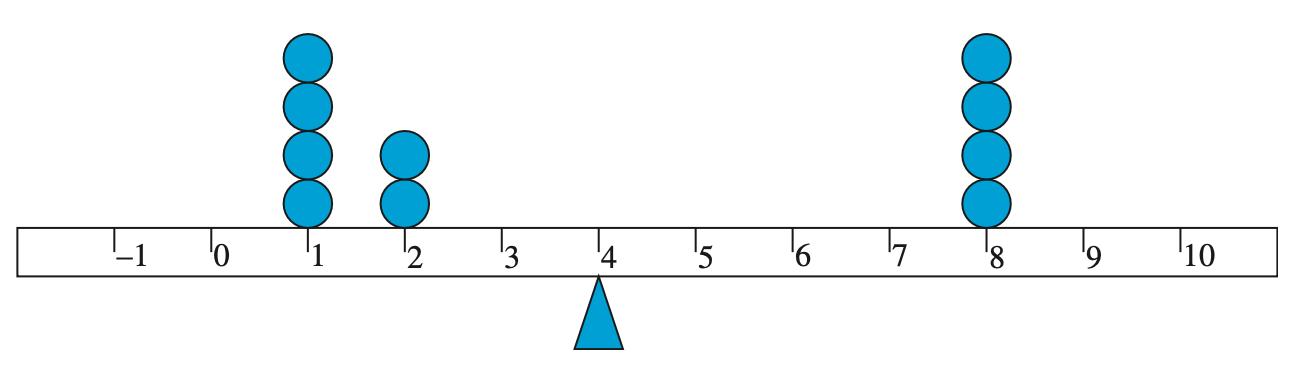
\includegraphics[width=.7\textwidth]{images/center_of_mass}
\end{figure}
\vfill 

To be concrete, the expected value for this problem is given by 
%
\begin{align*}
E[X] &= \sum_{a \in \R} a \, P(X=a) \\
&= 1 \times 0.4 + 2 \times 0.2 + 8 \times 0.4 \\
&= 4 
\end{align*}


\end{frame}


\begin{frame}
\small 

\begin{myredbox}[title=\text{Practice Reading Quiz (Expectation)}]


\begin{minipage}{.66\textwidth}
 Consider the spinner shown in the figure. Suppose that the likelihood of landing in each region is proportional to the area of the region.  Let $X$ be the number that appears on the spinner. Compute the expected value of $X$.
\end{minipage} %
\hfill 
\begin{minipage}{.28\textwidth}
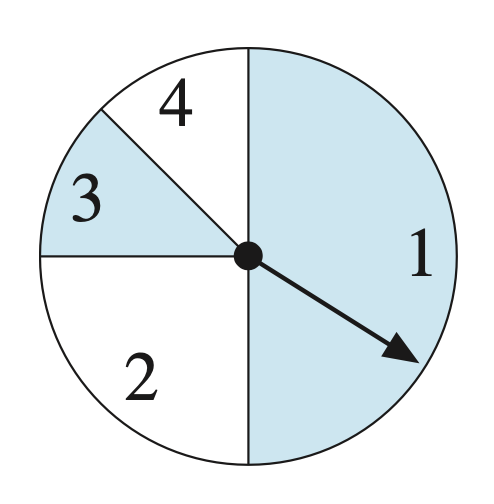
\includegraphics[width=\textwidth]{images/spinner.png}
\end{minipage}

\end{myredbox}
\vfill 
\pause 
\colorbox{green!30}{\textbf{Solution.}}
\[E[X] = \frac{1}{2} \cdot 1 + \frac{1}{4} \cdot 2 +   \frac{1}{8} \cdot 3 + \frac{1}{8} \cdot 4 = \frac{15}{8}.  \]
\vfill 
\pause 
\colorbox{blue!30}{\textbf{Remark.}} The expected value is a \textbf{weighted average}, where the weights are probabilities.


\end{frame}

%%%%%%%%%%%%%%%
%%%%%%%%%%%%%%%
%%%%%%%%%%%%%%%
\agendaframe{variance}

\begin{frame}{Variance as measure of spread}
\footnotesize 
\begin{mygreenbox}[title=Definition]
Let $X$ be a real-valued random variable on a probability space $(S,P)$. Let $\mu \defeq E[X]$.  Then the \textbf{variance} of $X$ is
\[ \Var(X) = \E \big[ (X - \mu)^2 \big] \]
\end{mygreenbox}

\vfill 

\begin{myredbox}[title=Remark]
The variance is the \textbf{expected squared deviation} from the mean. 
\end{myredbox}
\vfill 
\begin{figure}
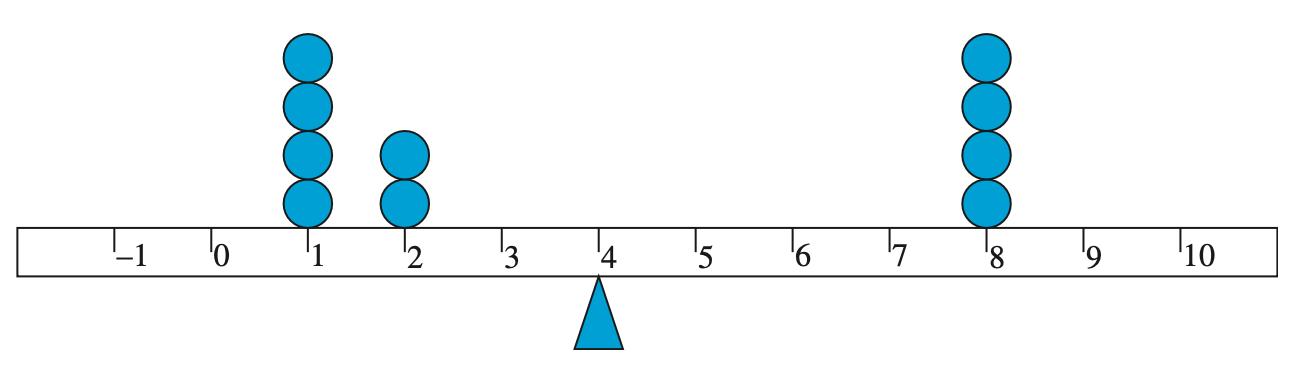
\includegraphics[width=.7\textwidth]{images/center_of_mass}
\end{figure}

\pause 
\vfill 
\colorbox{yellow!30}{\textbf{Poll.}} Can anybody here explain how to compute the variance for this problem? 
\end{frame}


\begin{frame}{Expectation vs. variance}
\footnotesize 
\begin{figure}
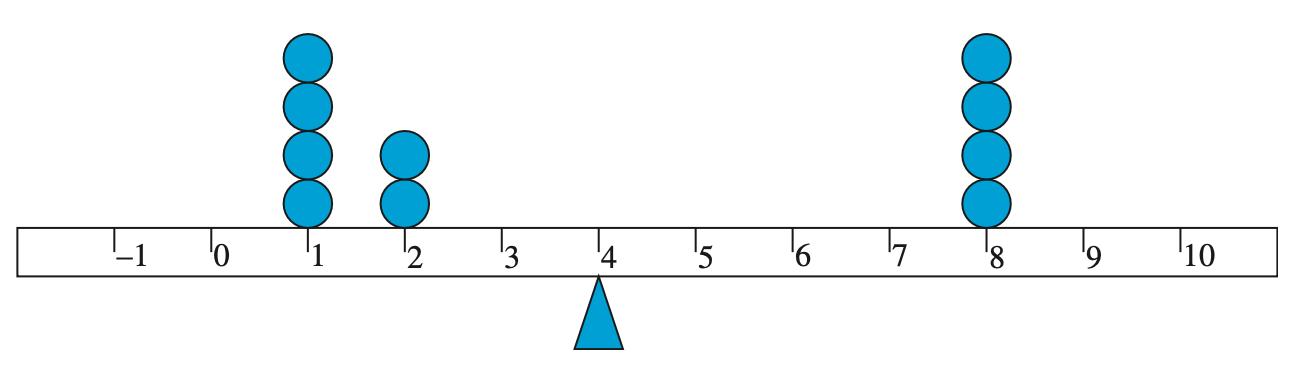
\includegraphics[width=.7\textwidth]{images/center_of_mass}
\end{figure}
\vfill 

Here, the \textbf{expected value} $E[X]$ (a.k.a. the mean $\mu$) is given by 
%
\begin{align*}
E[X] &= \sum_{a \in \R} \colorbox{yellow!30}{$a$} \, P(X=a) \\
&= \colorbox{yellow!30}{1} \times 0.4 + \colorbox{yellow!30}{2} \times 0.2 + \colorbox{yellow!30}{8} \times 0.4 \\
&= 4 
\end{align*}
%
\pause 
\vfill s
The \textbf{variance} $Var(X)$ (i.e. the expected squared deviation) is given by 
%
\begin{align*}
Var(X) &= \sum_{a \in \R} \colorbox{red!30}{$(a - \mu)^2$} \; P(X=a) \\
 &=\colorbox{red!30}{(1-4)^2} \times 0.4 + \colorbox{red!30}{(2-4)^2} \times 0.2 + \colorbox{red!30}{(8-4)^2} \times 0.4 \\
&= 9 \times 0.4 + 4 \times 0.2 + 16 \times 0.4 \\
&= 10.8
\end{align*}
%

\end{frame}

\begin{frame}
\footnotesize 

\begin{myredbox}[title=Remark]
When computing the variance, we can use
%
\begin{align*}
\Var(X) &= \sum_{s \in S} [X(s) - \mu]^2 \; P(s)  \\
\intertext{or}
&= \sum_{a \in \R} (a - \mu)^2 \; P(X=a)
\end{align*}
\end{myredbox}

\vfill 
\begin{figure}
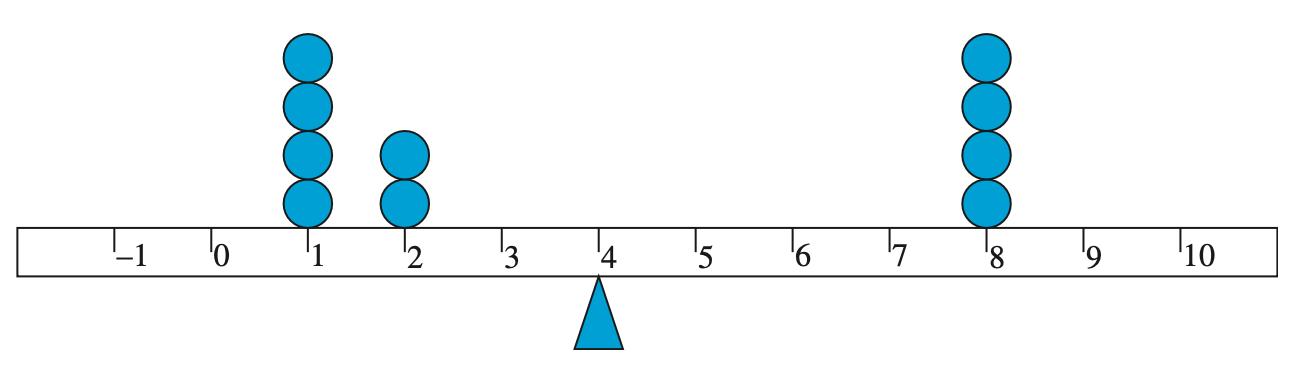
\includegraphics[width=.7\textwidth]{images/center_of_mass}
\end{figure}

\pause 
\vfill 
\colorbox{yellow!30}{\textbf{Poll.}} Can anybody explain how two apply these different methods to this problem?
\end{frame}



\begin{frame}{Three Random Variables}

\colorbox{yellow!30}{\textbf{Poll.}} These three random variables all have the same mean.  Which has the largest variance?
\vfill 
\centering
% Automatically scale to fit the width
\resizebox{\textwidth}{!}{
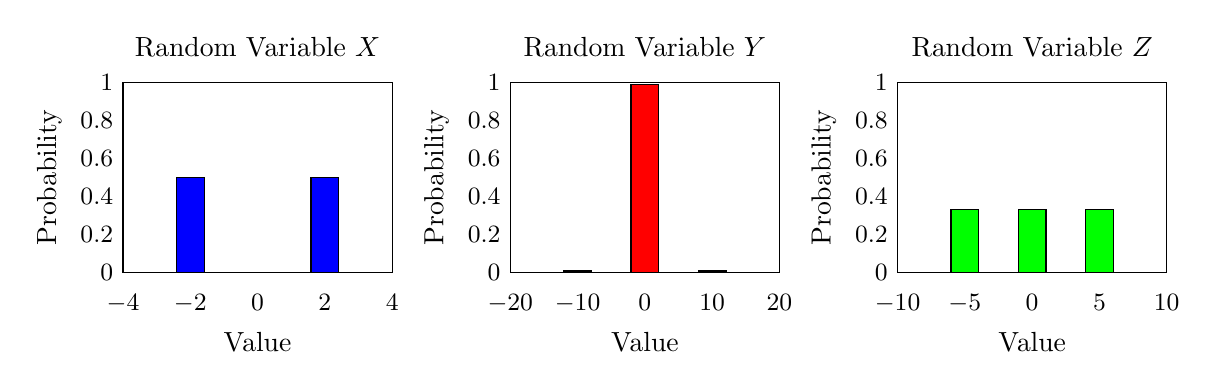
\begin{tikzpicture}
    % Group plots side by side
    \begin{groupplot}[
        group style={group size=3 by 1, horizontal sep=1.5cm},
        width=5cm, height=4cm,
        ybar,
        ymin=0, ymax=1,
        enlarge x limits=0.5,
        ylabel={Probability},
        xlabel={Value},
        xtick style={draw=none},
        ytick style={draw=none},
        xticklabel style={font=\small},
        yticklabel style={font=\small},
    ]

    % Histogram for X
    \nextgroupplot[title={Random Variable \(X\)}]
    \addplot[fill=blue] coordinates {(-2, 0.5) (2, 0.5)};

    % Histogram for Y
    \nextgroupplot[title={Random Variable \(Y\)}]
    \addplot[fill=red] coordinates {(-10, 0.01) (0, 0.99) (10, 0.01)}; 


    % Histogram for Z
    \nextgroupplot[title={Random Variable \(Z\)}]
    \addplot[fill=green] coordinates {(-5, 0.333) (0, 0.333) (5, 0.333)};

    \end{groupplot}
\end{tikzpicture}
}
\vfill
\pause 
\colorbox{blue!30}{\textbf{Solution.}} $Z$ has the largest variance. (See textbook for more info.)
 


\end{frame}






\begin{frame}[standout]
Group exercises
\end{frame}

\begin{frame}{Random group assignments}
\begin{columns}
\begin{column}{0.33\textwidth}
Ashley, Isabelle: 10 \\ 
Bailey, Tanna: 11 \\ 
Blaisdell, Olyver: 1 \\ 
Brown, Ashton: 10 \\ 
Cardenas, Dominic: 4 \\ 
Cutler, George: 1 \\ 
Fabik, Roland: 11 \\ 
Fellows, Audrey: 3 \\ 
Fitzgerald, Ryan: 9 \\ 
Fuller, Ryan: 10 \\ 
Griffen, Clara: 12 \\ 
Grutsch, Tanner: 8 \\\end{column}
\begin{column}{0.33\textwidth}
Hager, Nathan: 3 \\ 
Horner, Jayden: 4 \\ 
Johnson, Jaret: 7 \\ 
Kintzel, Samantha: 9 \\ 
Lameres, Alexis: 8 \\ 
Lee, Holden: 6 \\ 
Mayala, Reece: 11 \\ 
McLean, Connor: 5 \\ 
Mcbride, Daniel: 2 \\ 
Miller, Maverick: 5 \\ 
Moss, Emily: 2 \\ 
Mousseau, Matthew: 7 \\\end{column}
\begin{column}{0.33\textwidth}
Neuman, Evan: 6 \\ 
Putnam, John: 7 \\ 
Ramos, Vydel: 3 \\ 
Rathbun, Jedidiah: 8 \\ 
Roberts, Matthew: 1 \\ 
Roller, Nathan: 5 \\ 
Ryan, Otis: 12 \\ 
Shevtsov, Timothy: 4 \\ 
Stensland, Emma: 6 \\ 
Thiessen, Logan: 2 \\ 
Thompson, Jaiden: 9 \\ 
Vath, Ethan: 12 \\\end{column}
\end{columns}
\end{frame}

\begin{frame}{Group exercises}
\footnotesize 
\begin{enumerate}
	\item \textit{Simplified stock market.} Suppose there are three kinds of days: \texttt{GOOD}, \texttt{GREAT}, and \texttt{ROTTEN}. The following chart gives the frequency of each of these types of days and the effect on the price (in dollars) of a certain stock that day.
	
	\begin{table}[H]
	\begin{tabular}{|c|c|c|}
	\toprule 
	\colorbox{blue!30}{Type of day} & 	\colorbox{blue!30}{Frequency} & \colorbox{blue!30}{Change in stock value} \\
	\midrule 
	\texttt{GOOD} & 60\% & +2 \\
	\texttt{GREAT} & 10\% & +5 \\
	\texttt{ROTTEN} & 30\% & -4 \\
	\bottomrule 
	\end{tabular}
	\end{table}
	Assume the type of a given day is independent of the type of any other day.
	Let $X_n$ be the change in the value of the stock after $n$ consecutive days.
	 \begin{itemize} \footnotesize 
	\item[a.] Find $E[X_1]$, the expected change in stock price after one day. 
	\item[b.] Find  $Var[X_1]$, the variance in the change in stock price after one day. 
	\item[c.] Find $E[X_5]$.
	\item[d.] Find $Var[X_5]$.
	\end{itemize}
	\vspace{-.2cm}
	\item  \leavevmode
	\begin{minipage}{.70\textwidth}
	\footnotesize  A pair of 25-sided dice is rolled. Let $X$ be the sum of the two numbers and $Y$ be the product. Find $E[X]$ and $E[Y]$.
	\end{minipage} %
	\hfill 
	\begin{minipage}{.15\textwidth}
	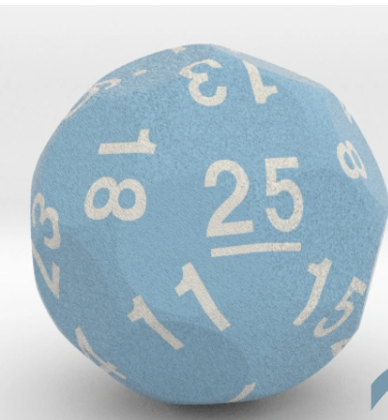
\includegraphics[width=.7\linewidth]{images/25_sided_die}
	\end{minipage}
	\vspace{-.1cm}
	\item  The term \textit{expected value} can be a bit deceiving. Sometimes it is not what someone might expect! (a) Give an example of a random variable $X$ where $E[X]=1$ but $P(X=1)=0$.  (b) Give an example of a random variable $X$ where $E[X]<0$ but the probability that $X$ is positive is nearly 100\%.
\end{enumerate}

\end{frame}


\begin{frame}{Solution to group exercise \#1a}
\footnotesize 

\textbf{Problem \& Solution.} \textit{Simplified stock market.} Suppose there are three kinds of days: \texttt{GOOD}, \texttt{GREAT}, and \texttt{ROTTEN}. The following chart gives the frequency of each of these types of days and the effect on the price (in dollars) of a certain stock that day.
	\vspace{-.2cm}
	\begin{table}[H]
	\begin{tabular}{|c|c|c|}
	\toprule 
	\colorbox{blue!30}{Type of day} & 	\colorbox{blue!30}{Frequency} & \colorbox{blue!30}{Change in stock value} \\
	\midrule 
	\texttt{GOOD} & 60\% & +2 \\
	\texttt{GREAT} & 10\% & +5 \\
	\texttt{ROTTEN} & 30\% & -4 \\
	\bottomrule 
	\end{tabular}
	\end{table}
	\vspace{-.2cm}
	Let $X_n$ be the change in the value of the stock after $n$ consecutive days.
		%
		\vspace{-.2cm}
		%
	 \begin{itemize} \footnotesize 
	\item[a.] Find $E[X_1]$, the expected change in stock price after one day. 
	%
	\begin{align*}
	 E[X_1] &= \sum_{s \in S} X_1(s) P(s)  \\
	 &= (+2)(0.6) + 	(+5)(0.1) + (-4)(.30) = 0.5
	\end{align*}
	%
	We expect the stock value to rise \$0.50 after one day.
	\end{itemize}
\end{frame}


\begin{frame}{Solution to group exercise \#1b}
\footnotesize 

\textbf{Problem \& Solution.} \textit{Simplified stock market.} Suppose there are three kinds of days: \texttt{GOOD}, \texttt{GREAT}, and \texttt{ROTTEN}. The following chart gives the frequency of each of these types of days and the effect on the price (in dollars) of a certain stock that day.
	\vspace{-.2cm}
	\begin{table}[H]
	\begin{tabular}{|c|c|c|}
	\toprule 
	\colorbox{blue!30}{Type of day} & 	\colorbox{blue!30}{Frequency} & \colorbox{blue!30}{Change in stock value} \\
	\midrule 
	\texttt{GOOD} & 60\% & +2 \\
	\texttt{GREAT} & 10\% & +5 \\
	\texttt{ROTTEN} & 30\% & -4 \\
	\bottomrule 
	\end{tabular}
	\end{table}
	\vspace{-.2cm}
	Let $X_n$ be the change in the value of the stock after $n$ consecutive days.
		%
		\vspace{-.2cm}
		%
	 \begin{itemize} \footnotesize 
	\item[b.] Find  $Var[X_1]$, the variance in the change in stock price after one day.
	%
	\begin{align*}
	 Var[X_1] &= \sum_{s \in S} (X_1(s)-\mu)^2 P(s)  && \text{(where $\mu \defeq \E[X_1]$)} \\
	 \intertext{Since we know from part (a) that $\mu=0.5$,}
	 &= \sum_{s \in S} (X_1(s)-0.5)^2 P(s) \\
	 &= (2 - 0.5)^2 \times .6 + 	(5-0.5)^2 \times .3 + (-4-0.5)^2 \times .10 \\
	 &= 9.45
	\end{align*}
	\end{itemize}
\end{frame}


\begin{frame}{Solution to group exercise \#1b -- Alternate solution.}
\footnotesize 

\textbf{Problem \& Solution.} \textit{Simplified stock market.} Suppose there are three kinds of days: \texttt{GOOD}, \texttt{GREAT}, and \texttt{ROTTEN}. The following chart gives the frequency of each of these types of days and the effect on the price (in dollars) of a certain stock that day.
	\vspace{-.2cm}
	\begin{table}[H]
	\begin{tabular}{|c|c|c|}
	\toprule 
	\colorbox{blue!30}{Type of day} & 	\colorbox{blue!30}{Frequency} & \colorbox{blue!30}{Change in stock value} \\
	\midrule 
	\texttt{GOOD} & 60\% & +2 \\
	\texttt{GREAT} & 10\% & +5 \\
	\texttt{ROTTEN} & 30\% & -4 \\
	\bottomrule 
	\end{tabular}
	\end{table}
	\vspace{-.2cm}
	Let $X_n$ be the change in the value of the stock after $n$ consecutive days.
		%
		\vspace{-.2cm}
		%
	 \begin{itemize} \footnotesize 
	\item[b.] Find  $Var[X_1]$, the variance in the change in stock price after one day.
	%
	\begin{align*}
	 Var[X_1] &= E[X_1^2] - E[X_1]^2
	 \end{align*}
	 %
	For the first summand,  
	%
	\begin{align*}
	E[X_1^2] &= \sum_{s \in S} X_1(s) P(s)  \\
	 &= (+2)^2 \times .6 + 	(+5)^2 \times .10 + (-4)^2 \times .30 = 0.5 \\
	 &= 4 \times .6 + 	25 \times .10 + 16 \times .30 = 9.7 
	 \end{align*}
	 %
	 For the second summand, we know  from part (a) that $\E[X_1]=0.5$. Hence $\E[X_1]^2=0.25$.  Putting this together, we have
	 \[  Var[X_1] = E[X_1^2] - E[X_1]^2 = 9.7-0.25 = 9.45.\]
	\end{itemize}
\end{frame}


\begin{frame}{Solution to group exercise \#1c}
\footnotesize 

\textbf{Problem \& Solution.} \textit{Simplified stock market.} Suppose there are three kinds of days: \texttt{GOOD}, \texttt{GREAT}, and \texttt{ROTTEN}. The following chart gives the frequency of each of these types of days and the effect on the price (in dollars) of a certain stock that day.
	\vspace{-.2cm}
	\begin{table}[H]
	\begin{tabular}{|c|c|c|}
	\toprule 
	\colorbox{blue!30}{Type of day} & 	\colorbox{blue!30}{Frequency} & \colorbox{blue!30}{Change in stock value} \\
	\midrule 
	\texttt{GOOD} & 60\% & +2 \\
	\texttt{GREAT} & 10\% & +5 \\
	\texttt{ROTTEN} & 30\% & -4 \\
	\bottomrule 
	\end{tabular}
	\end{table}
	\vspace{-.2cm}
	Let $X_n$ be the change in the value of the stock after $n$ consecutive days.
		%
		\vspace{-.2cm}
		%
	 \begin{itemize} \footnotesize 
	\item[c.] Find $E[X_5]$, the expected change in stock price after five days. 
	%
	The analysis is simplest if we write $X_5 = Y_1 + Y_2 + \hdots + Y_5$, where $Y_j$ is the change in stock price on the $j$-th day. \\
	
	Now, by linearity of expectation
	\[E[X_5] = E[Y_1] + E[Y_2] + \hdots + E[Y_5].\] 
	 %
	 Each summand is given by
	 \[E[Y_j] = (+2)(0.6) + 	(+5)(0.1) + (-4)(.30) = 0.5, \]
	 as was solved in part (a).
	 
	 Hence, 
	 \[E[X_5] = 5(0.5) = 2.5 \]
	  %
	  We expect the stock value to rise \$2.50 after 5 days.
	\end{itemize}
\end{frame}

\begin{frame}{Solution to group exercise \#1d}
\footnotesize
\textbf{Problem.}  Find $Var[X_5]$, the variance of the change in stock price after five days. 
\vfill \vfill 
\textbf{Solution.}   We write
  \[ Var[X_5] = E[X_5^2] - E[X_5]^2 \]
  For the second summand, we know from part (c) that $E[X_5] = 2.5$, so $ E[X_5]^2 = 2.5^2 = 6.25$. \\
   \vfill 
   For the first summand, we again write $X_5 = Y_1 + Y_2 + \hdots + Y_5$, where $Y_j$ is the change in stock price on the $j$-th day.  We use the fact that the $Y_j$'s are independent.
   %
   \begin{align*}
   E[X_5^2] &= E[(Y_1 + Y_2 + \hdots + Y_5)^2] \\
   &=E[Y_1^2 + \hdots + Y_5^2 + 2Y_1Y_2 + \hdots +2Y_4Y_5] && \scripttext{(expanding the sum of squares)}\\
   &= 5E[Y_1^2] + 20E[Y_1Y_2] && \scripttext{(since $Y_j$'s are identical)}\\
   &= 5E[Y_1^2] + 20E[Y_1]E[Y_2]  && \scripttext{(by independence)}\\
   &= (5)(9.7)  + 20(0.5)^2 && \scripttext{(using previous parts)}\\
   &= 53.5
   \end{align*}

Hence,
  \[ Var[X_5] = E[X_5^2] - E[X_5]^2 = 53.5 - 6.25 = 47.25 \]
\vfill \vfill 
\textbf{Remark.} This problem is much simpler if we use a fact (not presented in the text) that 
\[ Var(X_5) = Var(Y_1) + \hdots Var(Y_5)\]
because the $Y_j$'s are independent.
\end{frame}



\begin{frame}{Solution to group exercise \#2}
\footnotesize 
\textbf{Problem.} A pair of 25-sided dice is rolled. Let $X$ be the sum of the two numbers and $Y$ be the product. Find $E[X]$ and $E[Y]$.
\vfill 
\textbf{Solution.} Let $X_i$ be the value of the die on the $i$-th roll, where $i \in \set{1,2}$.   \\

Now $X=X_1+X_2$. So by linearity of expectation, $E[X]=E[X_1]+E[X_2]$.  Each $X_i$ satisfies
%
\begin{align*}
E[X_i] &= \sum_{s \in S} X(s) P(s) \\
&= (1+\hdots + 25) \frac{1}{25} \\
&= \frac{(25)(26)}{2} \frac{1}{25} \\
&=13
\end{align*}
Hence
\[E[X]=E[X_1]+E[X_2] = 13+13 =26 \]
So on average, the sum of the values on the two dice will be 26. \\
\vfill 
Moreover $Y=X_1 X_2$. By independence, $E[Y] = E[X_1]E[X_2]$.  So the expected product of the two rolls is
\[E[Y]=E[X_1]E[X_2] = (13)(13) = 169. \]
So on average, the product of the values on the two dice will be 169. \\

\end{frame}

\begin{frame}{Solution to group exercise \#3}
\footnotesize

\textbf{Problem.} The term \textit{expected value} can be a bit deceiving. Sometimes it is not what someone might expect! (a) Give an example of a random variable $X$ where $E[X]=1$ but $P(X=1)=0$.  (b) Give an example of a random variable $X$ where $E[X]<0$ but the probability that $X$ is positive is nearly 100\%.
\vfill 
\textbf{Solution.}
\begin{itemize}
\item[a.] Let $X$ be a random variable that takes on the value $X=2$ with probability $\frac{1}{2}$ and the value $X=0$ with probability $\frac{1}{2}$. Then
\[ E[X] = \sum_{a \in \R} a \, P(X=a) = \bigg(\half \bigg)(0) + \bigg(\half \bigg)(2) = 1. \]
But $P(X=1)=0$.
\item[b.] Let $X$ be a random variable that takes on the value $X= -1,000,000$ with probability $0.001$ and the value $X=1$ with probability $0.999$.
Then 
\[ E[X] = \sum_{a \in \R} a \, P(X=a) = (.001)(-1,000,000) + (.999)(1) = -999.001. \]
So $E[X]<0$; that is, the expected value  of the random variable is negative. But 
\[P(X>0)=P(X=1)= 0.999\]
So the probability that $X$ is positive is almost 100\%.
\end{itemize}
	
\end{frame}


\end{document}
